\documentclass[a4paper]{article}
\usepackage[pdftex]{graphicx}
\usepackage[utf8]{inputenc}
\usepackage{enumerate}
\usepackage{icomma}
\usepackage{siunitx}
\sisetup{locale=DE}
\usepackage{amssymb}
\usepackage{tikz}
\usepackage{href-ul}
\hypersetup{
	colorlinks=true,
	linkcolor=blue,
	urlcolor=blue}
\usepackage{geometry}
\geometry{a4paper, top=15mm, left=15mm, right=15mm, bottom=15mm,
	headsep=10mm, footskip=12mm}

\begin{document}
	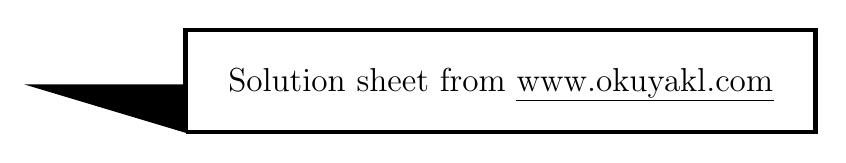
\begin{tikzpicture}(10,3)
		\draw[ultra thick](2,0) --(10,0) -- (10,1.3) --(2,1.3) -- (2,0);
		\draw[fill=black](2,0)-- (0,.6) -- (2,.6) -- (2,0);
		\node at (6,.6) {\large Solution sheet from \href{http://www.okuyakl.com}{www.okuyakl.com}};
	\end{tikzpicture}
	\vspace{0.5 cm}
	
	\noindent{\bf Task 1. a)}\\
	$r=d/2 = \SI{14}{\milli\meter}$; \qquad $O=4 \pi r^2 = \SI{2463}{\milli \meter^2} \approx \SI{24,6}{\centi \meter^2}$
	
	\noindent{\bf Task 1. b)}\\
	$$
	\renewcommand{\arraystretch}{2}
	\begin{array}{rcll}
		O&=& 4\pi r^2 &|:4 \pi \\
		{O\over 4\pi} &=& r^2 &|\sqrt{\quad}\\
		\sqrt{O\over 4\pi} &=& r\\
		r&=& \sqrt{\SI{100}{\centi\meter^2} \over 4 \pi} &= \SI{2.82}{\centi\meter}\\
		d&=& 2\cdot \SI{2.82}{\centi\meter} &= \SI{5.64}{\centi\meter}
	\end{array}
	$$
	\noindent{\bf Task 1. c)}\\
	$d=2r=\SI{11.78}{\meter}$; \qquad $O= 4 \pi r^2 = \SI{436}{\meter^2}$
	
	\noindent{\bf Task 2.}\\
	We set $V=O$ and solve for $r$:
	$$
	\renewcommand{\arraystretch}{2}
	\begin{array}{rcll}
		4\pi r^2 &=& {4 \over 3} \pi r^3 &| :4\pi\\
		r^2 &=& {1 \over 3} r^3 &| \cdot 3 : r^2\\
		3 &=& r
	\end{array}
	$$
	If the radius of a sphere is 3 units of length, then the measure of the area is equal to that of the volume:
	$V=O=36\pi$.
	
	\noindent{\bf Task 3.}\\
	We imagine a ball that just fits into a cube. Then the radius of the sphere is $r$ and the edge length of the cube is $2r$. The surface of the sphere is then $O_K$, the surface of the cube is $O_W$; the following applies:
	
	$${O_W-O_K \over O_K}\cdot 100\% = {6\cdot (2r)^2 - 4\pi r^2 \over 4\pi r^2 }\cdot 100\% ={24 - 4 \pi \over 4\pi}\cdot 100\% = 91\%$$
	So the cube surface area is 91% larger, regardless of $r$.
	
	\noindent{\bf Task 4.}\\
	By rearranging the volume formula we get the radius:
	$$r=\sqrt[3]{V\cdot 3 \over 4 \pi} = \SI{11,15}{\centi\meter}$$
	We use this to calculate the surface area:
	$$O=4\pi r^2 = \SI{1561}{\centi\meter^2}$$
	For example, a rectangle with the same area would have the dimensions:
	$$\SI{1561}{\centi\meter^2} : \SI{50}{\centi\meter} = \SI{31}{\centi\meter}$$
	So it would be $\SI{50}{\centi\meter}$ long and $\SI{31}{\centi\meter}$ wide (The $\SI{50}{\centi\meter}$ are completely arbitrary chosen).
	
	\noindent{\bf Task 5. a)}\\
	The surface of this hemisphere is:
	$$O=2\pi r^2 = 2 \pi \cdot (\SI{20}{\meter})^2 = \SI{2513}{\meter^2}$$
	
	\noindent{\bf Task 5. b)}\\
	The volume of the installed glass is
	$$V= {m \over \varrho} = {240~t \over 2.4~t\cdot m^{-3}}=\SI{100}{\meter^3}$$
	We make the approximation that this volume is equal to the area times the glass thickness, then:
	$$ d = {V \over O}= {\SI{100}{\meter^3} \over \SI{2513}{\meter^2}} \approx \SI{0.04}{\meter} =\SI{4}{\centi\meter}$$
	
	\noindent{\bf Task 6.}\\
	The surface of the sphere with radius $r$ is:
	$$r= \sqrt[3]{3 V \over 4\pi} = \SI{4,9}{\centi\meter} \quad \Rightarrow \quad O= 4\pi r^2 = \SI{ 304}{\centi\meter^2}$$
	
	The hemispherical surface is with radius $r$:
	$$r= \sqrt[3]{3 V \over 2\pi} = \SI{6,2}{\centi\meter} \quad \Rightarrow \quad O= 2\pi r^2 + \pi r ^2= \SI{363}{\centi\meter^2}$$
	
	The cube surface with edge length $a$ is:
	$$a=\sqrt[3]{\SI{500}{\centi \meter^3}}=\SI{7,9}{\centi \meter} \quad \Rightarrow \quad O = 6r^2= \SI{378}{\centi\meter^2}$$
	
	We set the surface of the sphere = 100. The ratio of the surfaces is then sphere: hemisphere: cube
	$$100:119:124$$
	
	\noindent{\bf Task 7.}\\
	The radius $r$ increases by a tenth and is then $1.1~r$. The percentage increase in surface area is then calculated using the formula:
	$$({O_{new} \over O_{old}}-1)\cdot 100\% = ({4 \pi (1,1r)^2 \over 4 \pi r^2}-1)\cdot 100% =
	({1,1^2 \over 1}-1)\cdot 100\% = (1,21-1)\cdot 100\% = 21\%$$
	
	\noindent{\bf Task 8. a)}\\
	We calculate the volume of a grain of sand:
	$$V_s = {4 \over 3} \pi r^3 = {4 \over 3} \pi \cdot (\SI{0.5}{\milli\meter})^3 = \SI{0.52 }{\milli\meter^3}$$
	All grains of sand have the volume:
	$$V_a= {m \over \varrho}= \SI{100}{\centi \meter^3} = \SI{100000}{\milli \meter^3}$$
	We get the number of grains of sand by taking the quotient:
	$$n= {V_a \over V_s}= 190000$$
	We multiply this number by the diameter of a grain and find for the length l of the row of sand grains:
	$$ l = 190000 \cdot\SI{0.001}{\meter} = \SI{190}{\meter}$$
	 
\noindent{\bf Task 8. b)}\\
The surface of a grain of sand is:
$$O_s = 4\pi r^2 = 4 \pi \cdot (\SI{0.5}{\milli\meter})^2 = \SI{3.14}{\milli\meter^2} $$
The total surface area of the sand sample is:
$$O_a=n \cdot O_s = \SI{596903}{\milli\meter^2} \approx \SI{0.6}{\meter^2} $$

\noindent{\bf Task 8. c)}\\
Double the radius $\Rightarrow$ eight times the grain volume $\Rightarrow$ one eighth number of grains $\Rightarrow$
$$ l_d= l \cdot 2 \cdot {1\over 8} = {1\over 4}l$$
$\Rightarrow$ The length of the sand row is shortened to a quarter.

\noindent{\bf Task 8. d)}\\
Double the radius $\Rightarrow$ four times the grain surface, but here too we have 8 times fewer grains.
$$ \Rightarrow O_d = O \cdot 4 \cdot {1\over 8} = {1\over 2}O$$
$\Rightarrow$ The surface area of the sand decreases by half.

\noindent{\bf Task 9. a)}\\
The area of a small sunspot is
$$A_k=\pi r^2 = \pi \cdot (\SI{7,5}{\kilo\meter})^2 = \SI{350}{\kilo\meter^2} = \SI{3 .5e2}{\kilo\meter^2}$$
The area of a large sunspot is
$$A_g=\pi r^2 = \pi \cdot (\SI{75000}{\kilo\meter})^2 = \SI{3.50e10}{\kilo\meter^2}$$
The area can therefore be increased by a factor
$$ {A_g \over A_k} = 10^8$$
vary.

\noindent{\bf Task 9. b)}\\
The earth's surface is:
$$O_E=4\pi r^2 = 4 \pi \cdot (\SI{6370}{\kilo\meter})^2= \SI{5,1e8}{\kilo\meter^2}$$

A large sunspot is by the factor
$${A_g \over O_E} = 68 $$
larger than the surface area of the Earth.

\begin{center}
	\includegraphics[width=7 cm]{../../viecher/eendcomic.pdf}
	
	Here you can go back to the \href{https://www.okuyakl.de/math/m10kugobL218/ae218.pdf}{task sheet}
\end{center}

\end{document}